\begin{frame}\frametitle{Cut-Based Event Selection}
\begin{table}[h]
\scriptsize
\begin{center}
\begin{tabular}{|c|c|}
{\footnotesize\bfseries{- - - - - - - Muon Channel - - - - - - -}} & 
{\footnotesize\bfseries{- - - - - - Electron Channel - - - - - -}}\\ \hline
 {\scriptsize{HLT\_IsoMu24\_eta2p1}} &  {\scriptsize{HLT\_Ele27\_WP80}}  \\ \hline
 \multicolumn{2}{|c|}{Photon selection:}\\
 \multicolumn{2}{|c|}{\tiny{medium ID; $p_T>15$; $|\eta| < 1.4442$ or $1.566 < |\eta| < 2.5$}}\\ 
               &{\tiny{ ElectronConversionVeto$\rightarrow$PixelSeedVeto}} \\ \hline
 Muon tight ID & Electron tight ID \\ \hline
 \tiny{$p_T^{\mu}>25$ GeV;} &  \tiny{$p_T^{ele}>30$;}  \\ 
 \tiny{$|\eta^{\mu}|<2.1$} & \tiny{$|\eta^{ele}| < 1.4442$ or $1.566 < |\eta^{ele}| < 2.5$} \\ \hline
 \multicolumn{2}{|c|}{Second lepton veto:}\\
 \tiny{$p_T^{\mu2}>10$ GeV;} &  \tiny{$p_T^{ele2}>10$;} \\
 \tiny{$|\eta^{\mu2}|<2.4$}  &   \tiny{$|\eta^{ele2}| < 1.4442$ or $1.566 < |\eta^{ele2}| < 2.5$;} \\
  &   \tiny{veto ID for ele2} \\ \hline
 $M_T^W>40$ GeV & $M_T^W>40$ GeV \\ \hline
  & $110~GeV>M_{e\gamma}>70~GeV$ excluded \\ \hline
 \multicolumn{2}{|c|}{$\Delta{R}(lep,\gamma)>0.7$}\\  \hline
\end{tabular}
\end{center}
\end{table}

\end{frame}%{Cut-Based Event Selection}

%\begin{frame}\frametitle{Weights and Corrections}
%\begin{table}[h]
%\scriptsize
%\begin{center}
%\begin{tabular}{|c|c|}
%{\footnotesize\bfseries{- - - - - - - Correction - - - - - - -}} & 
%{\footnotesize\bfseries{- - - - - - - - Status - - - - - - - -}}\\ \hline
% luminosity reweight on MC & applied \\ \hline
% pileup reweight on MC & applied \\ \hline
% MET corrections and smearing & applied \\ \hline
% photon ID scale factors & applied \\ \hline
% PixelSeedVeto scale factors * & applied \\ \hline
% electron ID scale factors & applied \\ \hline
% muon ID scale factors & applied \\ \hline
%% $M^W_T$ scale factors & not applied \\ \hline
%% PHOSPHOR correction & not applied \\ \hline
%% (LO + up to 2 jets)/NLO on signal MC & negligible \\ \hline
%% NLO/NNLO on signal MC & not applied \\ \hline
%\end{tabular}
%\end{center}
%\end{table}
%\tiny
% * PixelSeedVeto scale factors are taken from the W$\gamma\gamma$ 8 TeV analysis\\
%- - - - - - - - - - - -\\
%\tiny 
%Number of vertices, Data vs MC plots. Z$\gamma$ selected sample, muon channel. \\
%Left: no PU reweighting applied, right: PU reweighting applied.
%\begin{figure}[htb]
%  \begin{center}
%   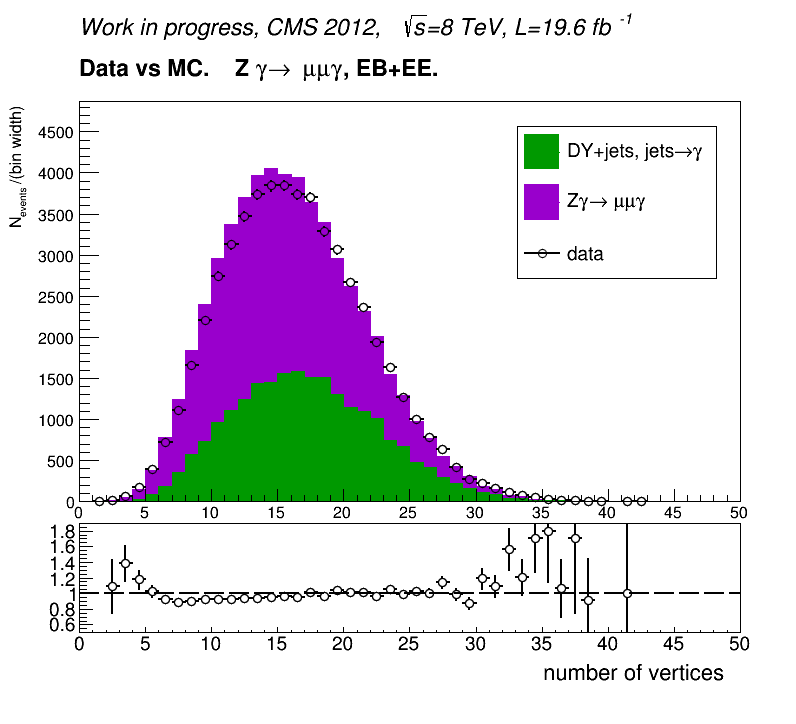
\includegraphics[width=0.5\textwidth]{../figs/figs_v11/MUON_ZGamma/PrepareYields/c_TotalDATAvsMC_EtaCommon__nVtx_noPU.png}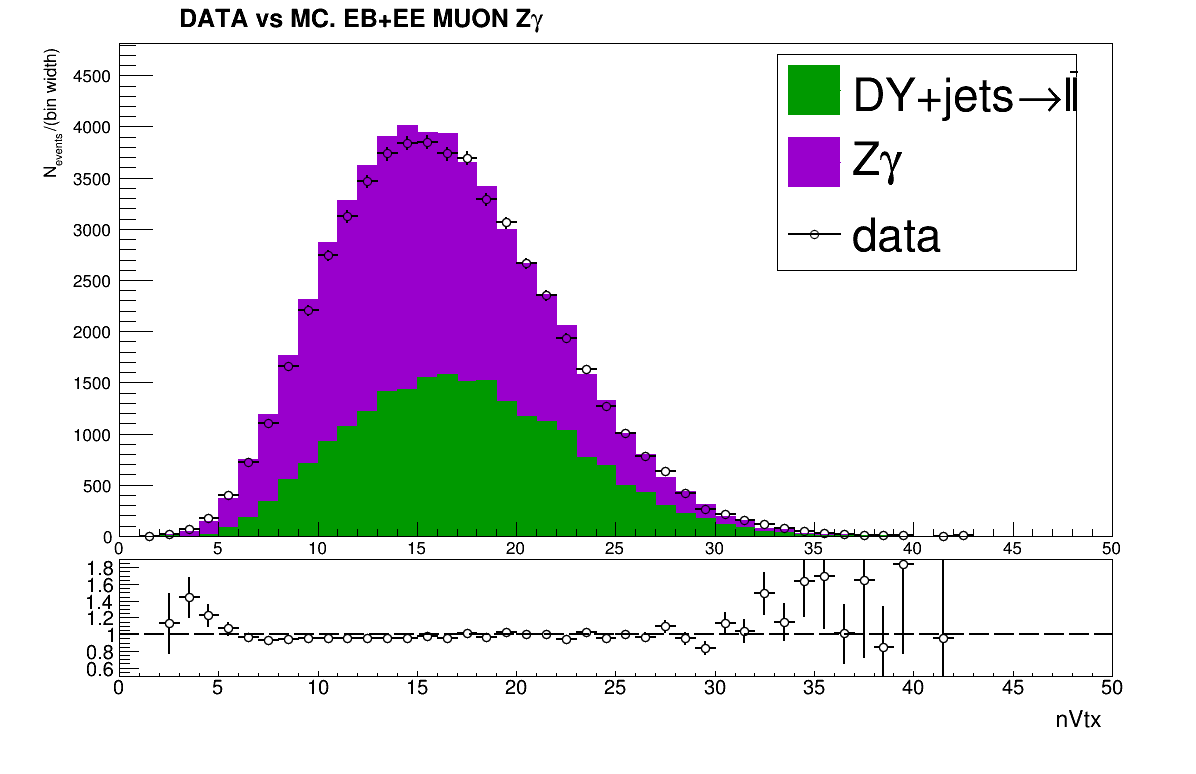
\includegraphics[width=0.5\textwidth]{../figs/figs_v11/MUON_ZGamma/PrepareYields/c_TotalDATAvsMC_EtaCommon__nVtx.png}
%  \label{fig:DATAvsMC_nVtx}
%  \end{center}
%\end{figure}
%\end{frame}

\begin{frame}\frametitle{Data vs MC. $P_T^{\gamma}$}
\scriptsize
  \begin{figure}[htb]
    \begin{center}
       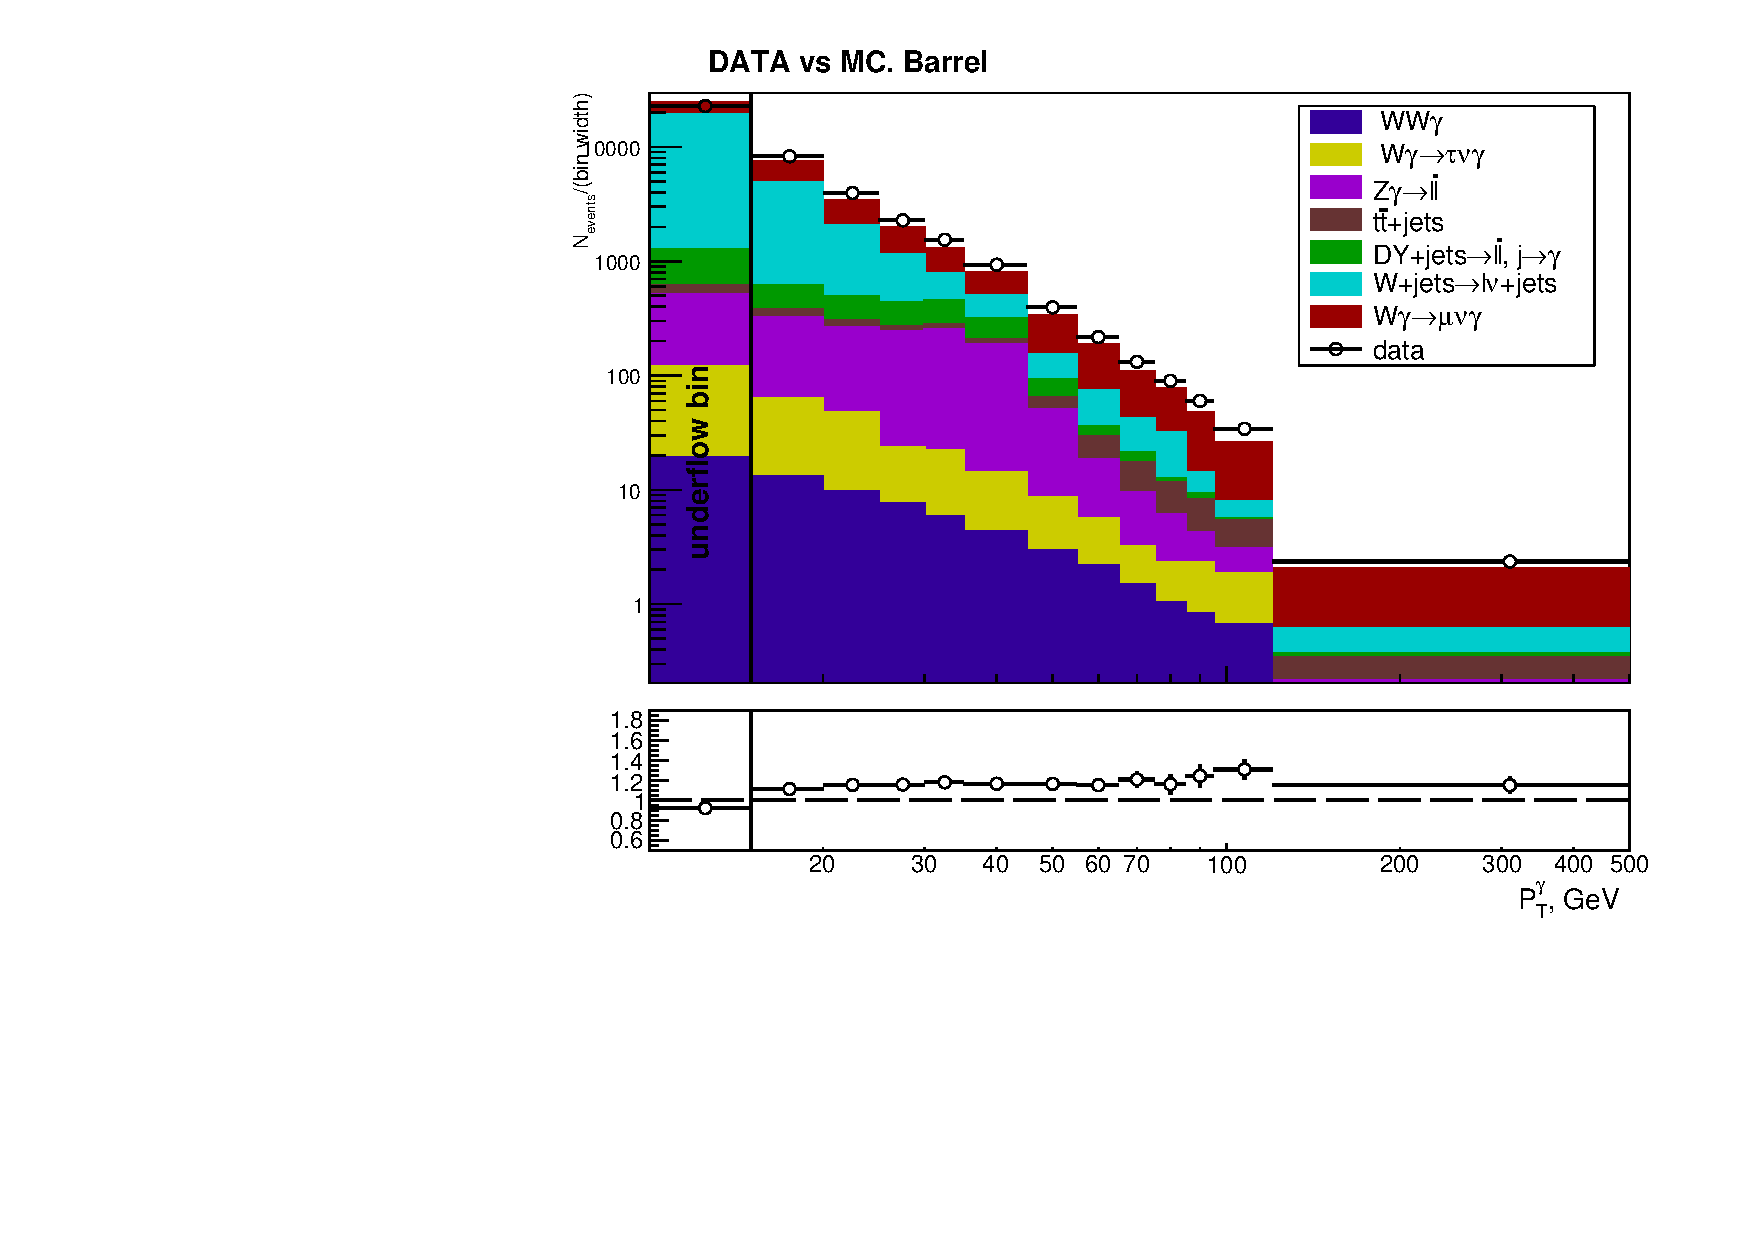
\includegraphics[width=0.5\textwidth]{../figs/figs_v11/MUON_WGamma/PrepareYields/c_TotalDATAvsMC_Barrel__phoEt.pdf} 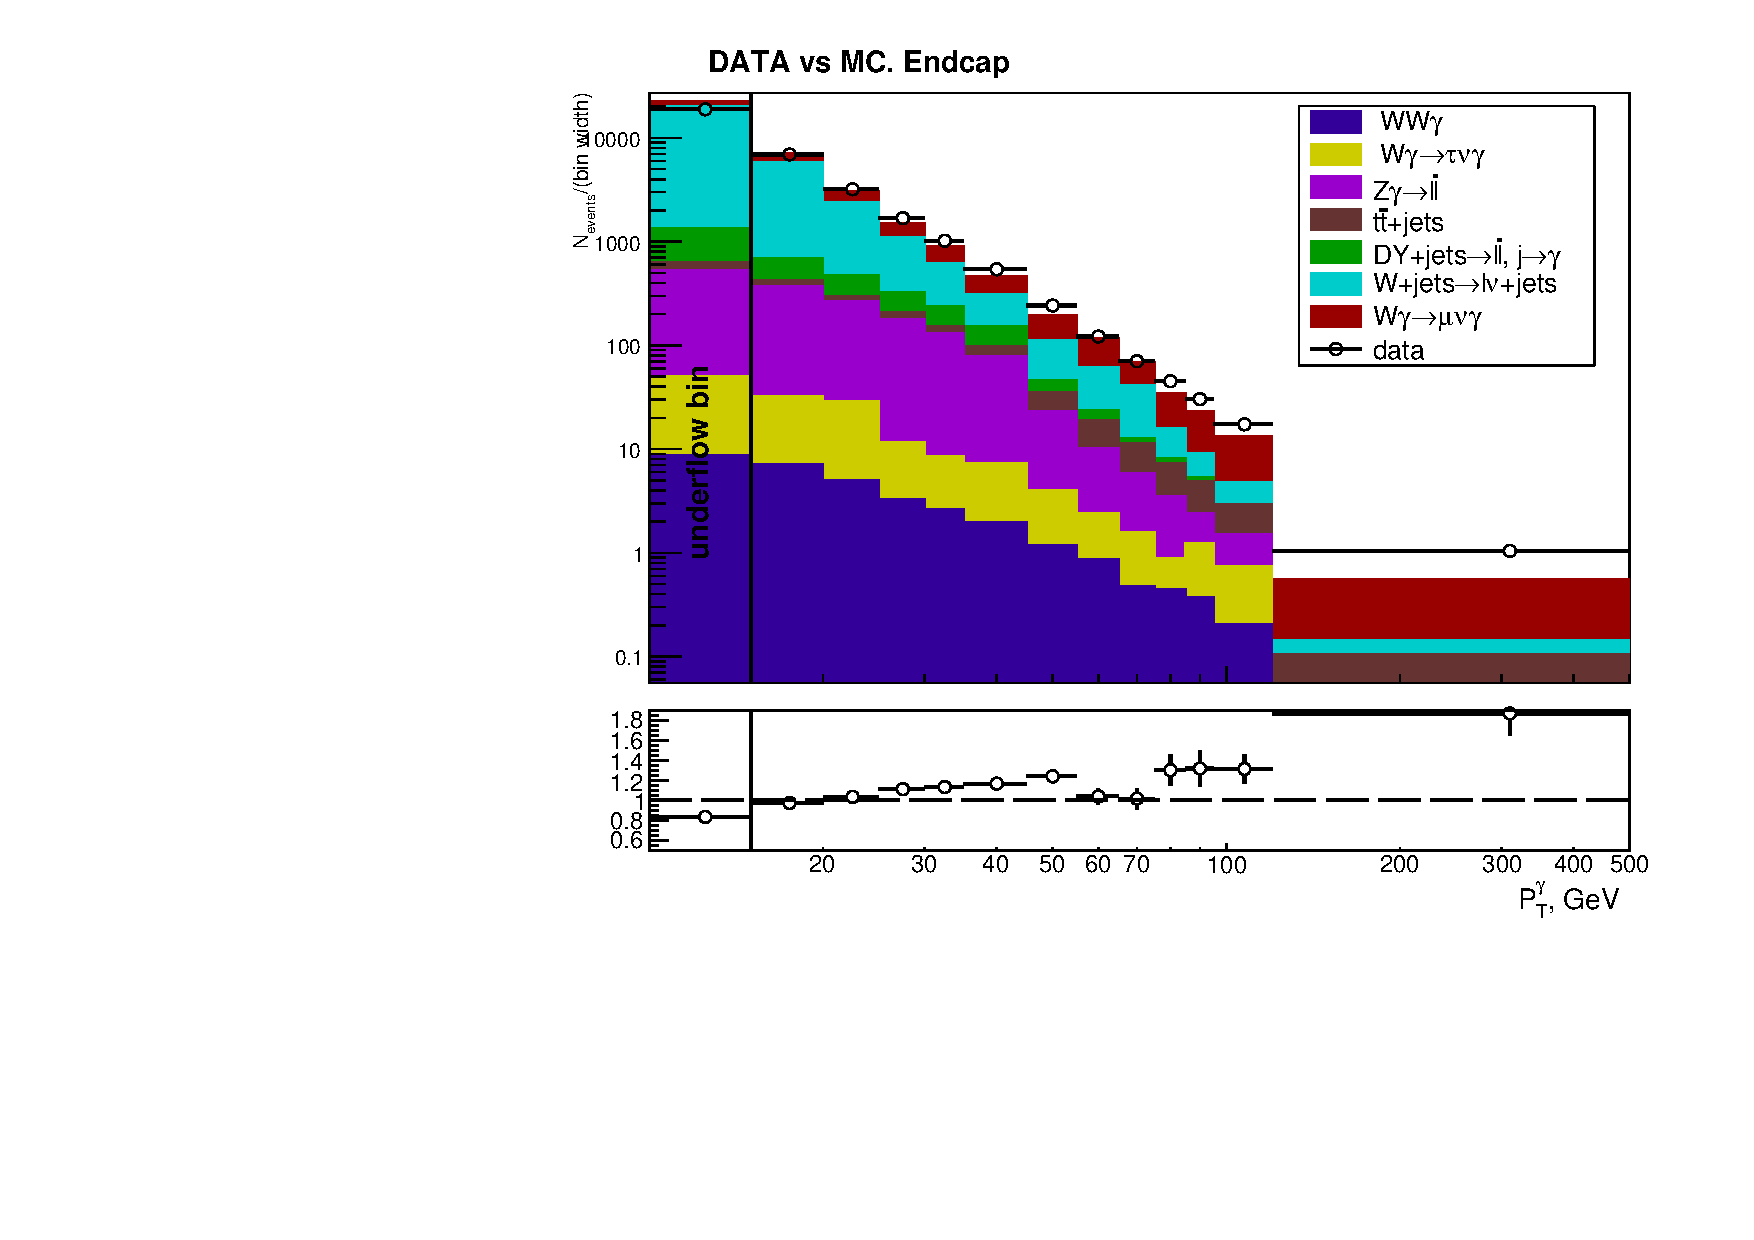
\includegraphics[width=0.5\textwidth]{../figs/figs_v11/MUON_WGamma/PrepareYields/c_TotalDATAvsMC_Endcap__phoEt.pdf}\\
       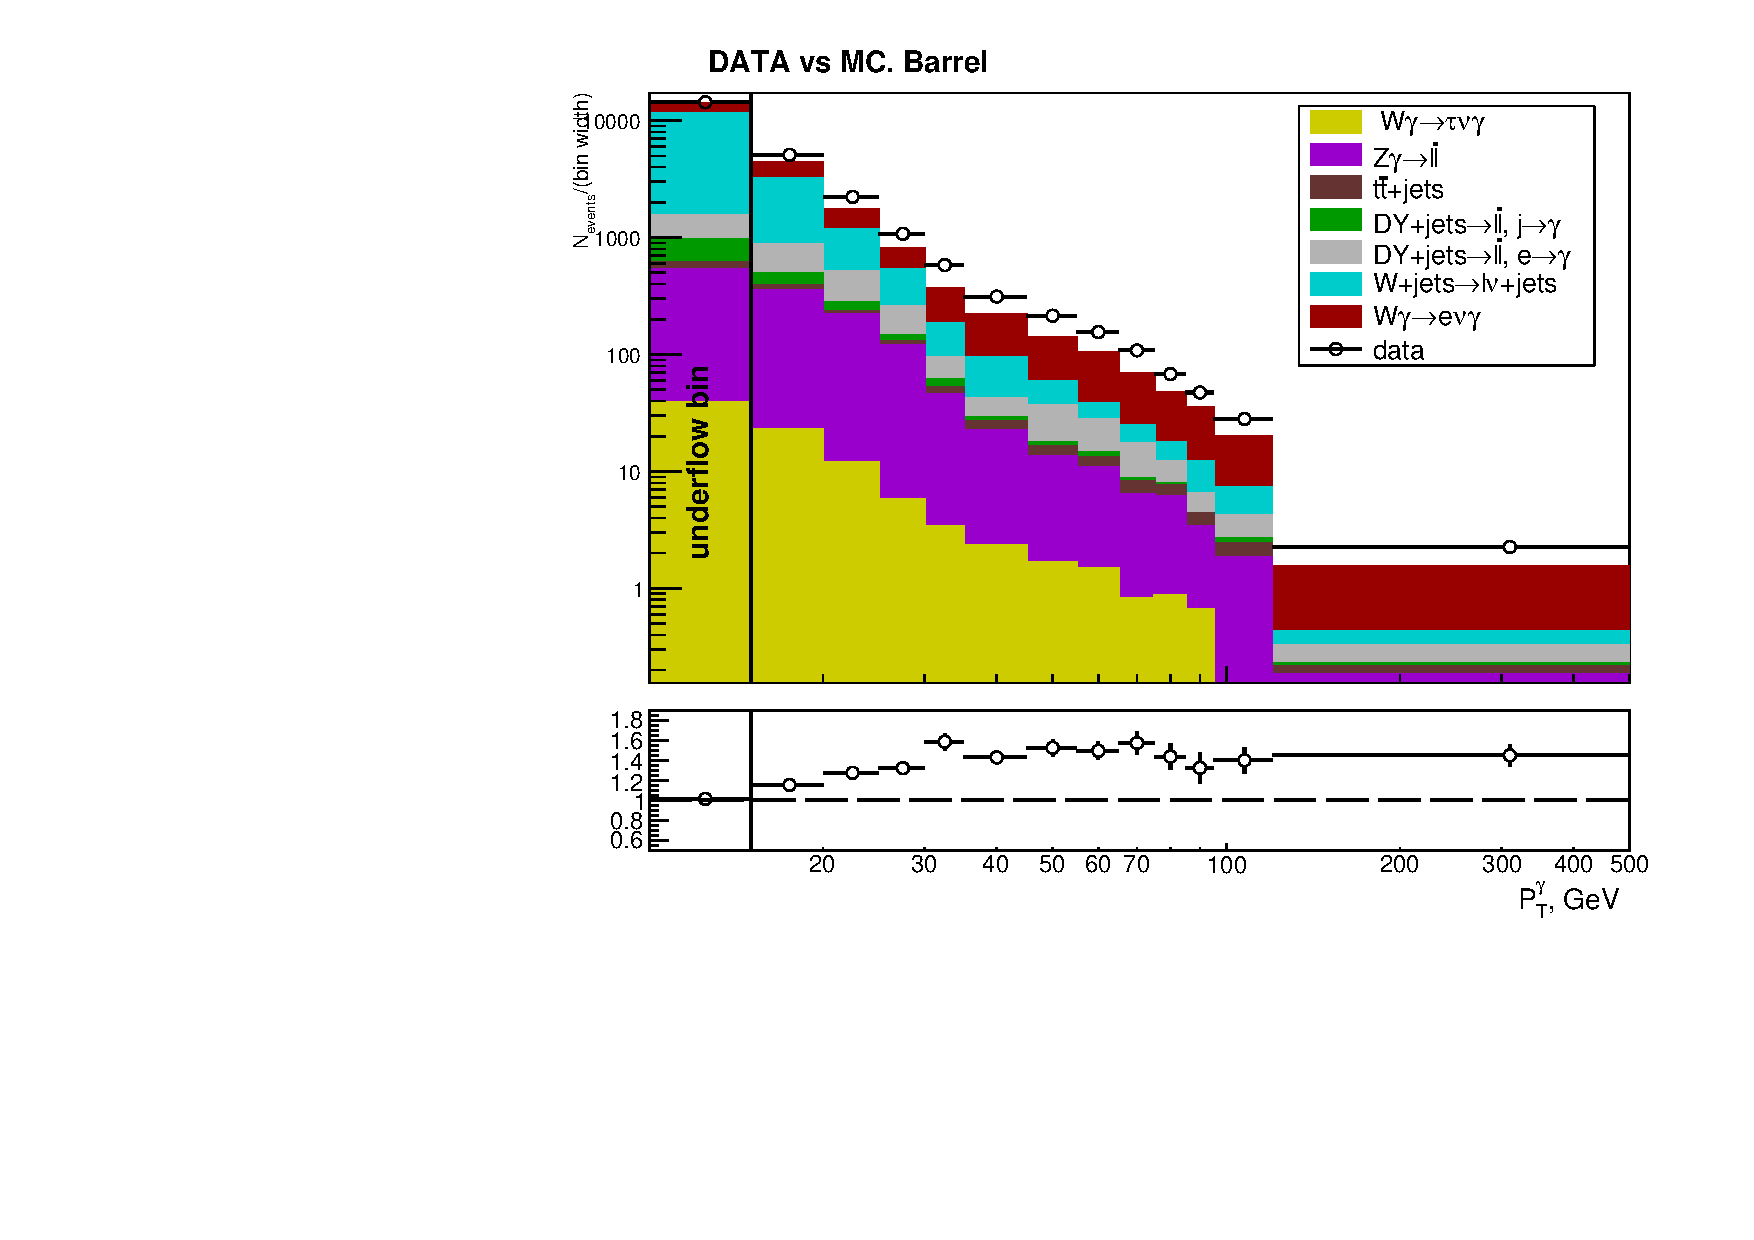
\includegraphics[width=0.5\textwidth]{../figs/figs_v11/ELECTRON_WGamma/PrepareYields/c_TotalDATAvsMC_Barrel__phoEt.pdf} 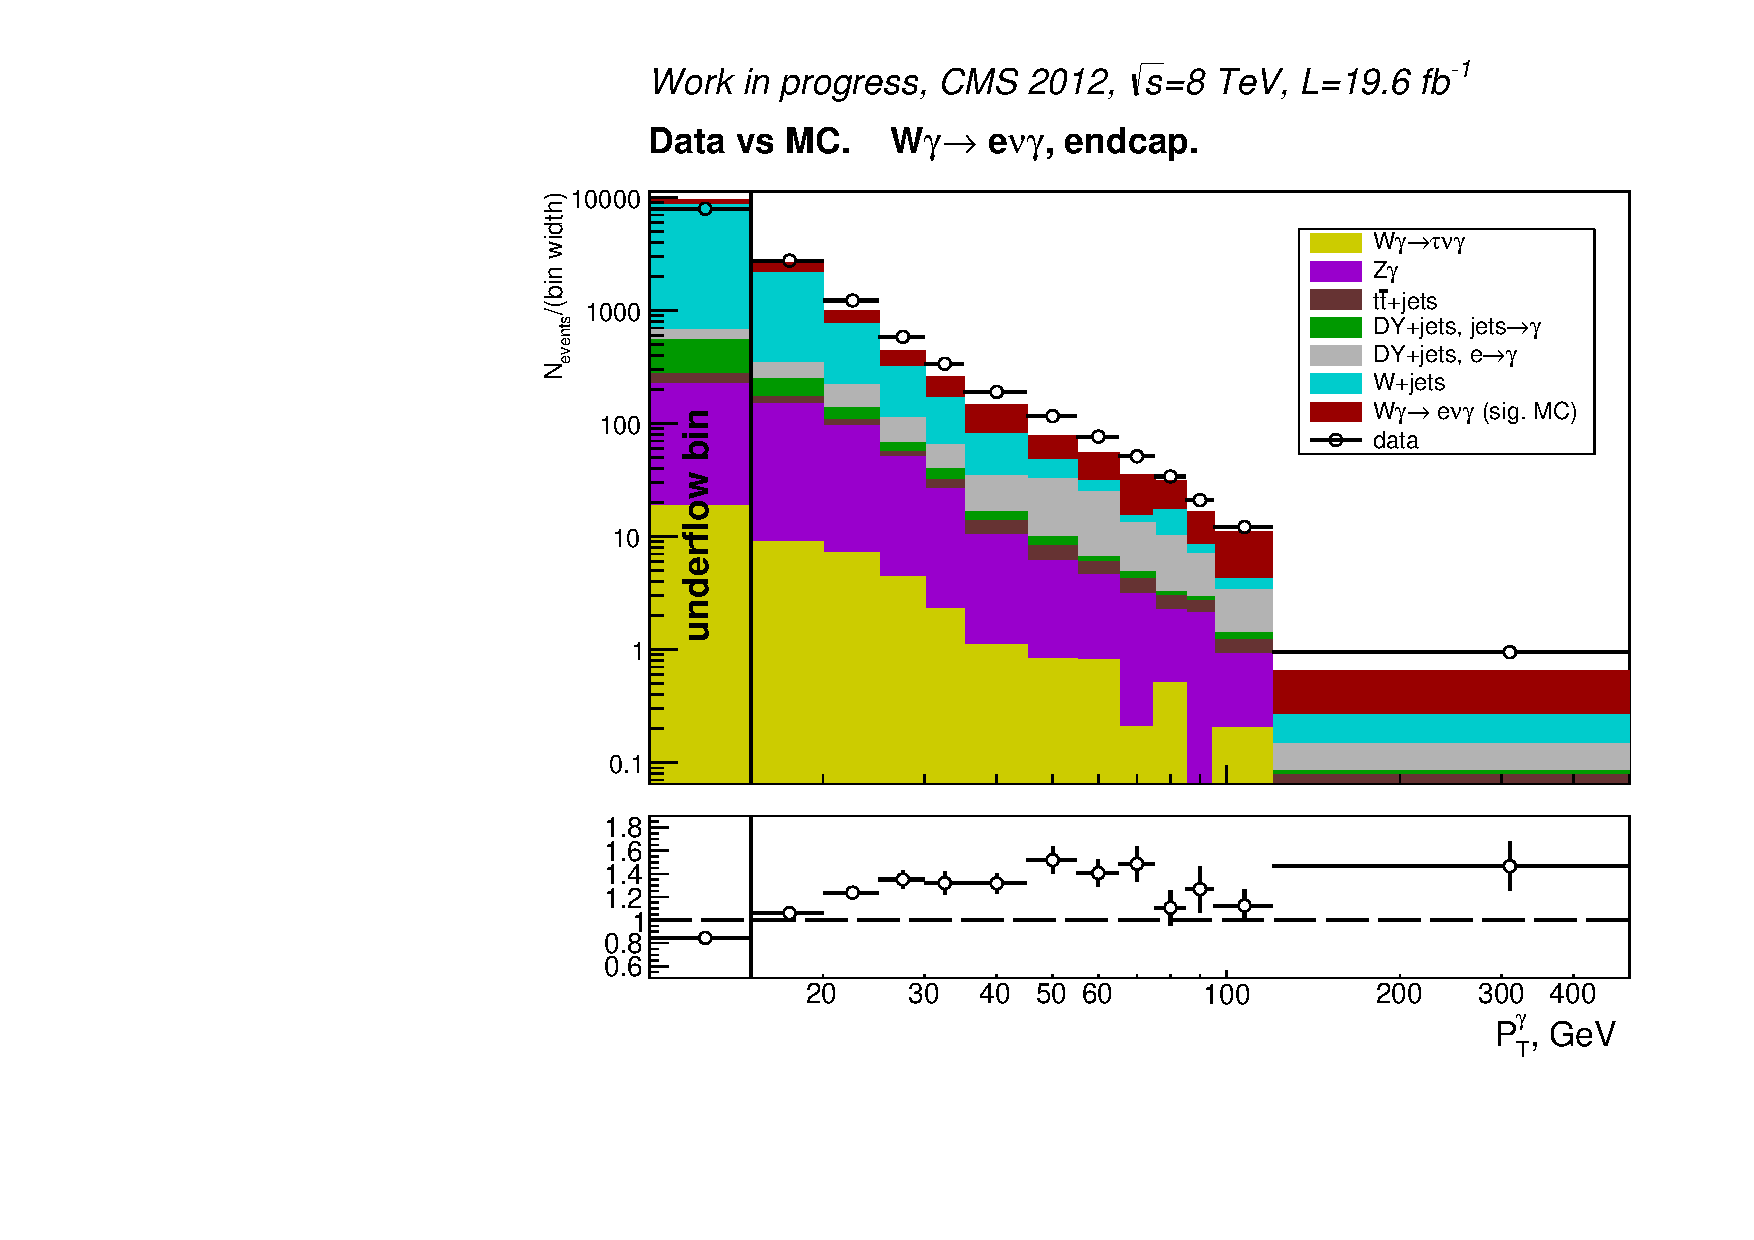
\includegraphics[width=0.5\textwidth]{../figs/figs_v11/ELECTRON_WGamma/PrepareYields/c_TotalDATAvsMC_Endcap__phoEt.pdf}\\
    \end{center}
  \end{figure}
\end{frame}

\begin{frame}\frametitle{Data vs MC. $M_T^W$}
\scriptsize
The selection requirement of {\bfseries{$M_T^W>40$~GeV}} is applied.
\begin{figure}[htb]
  \begin{center}
   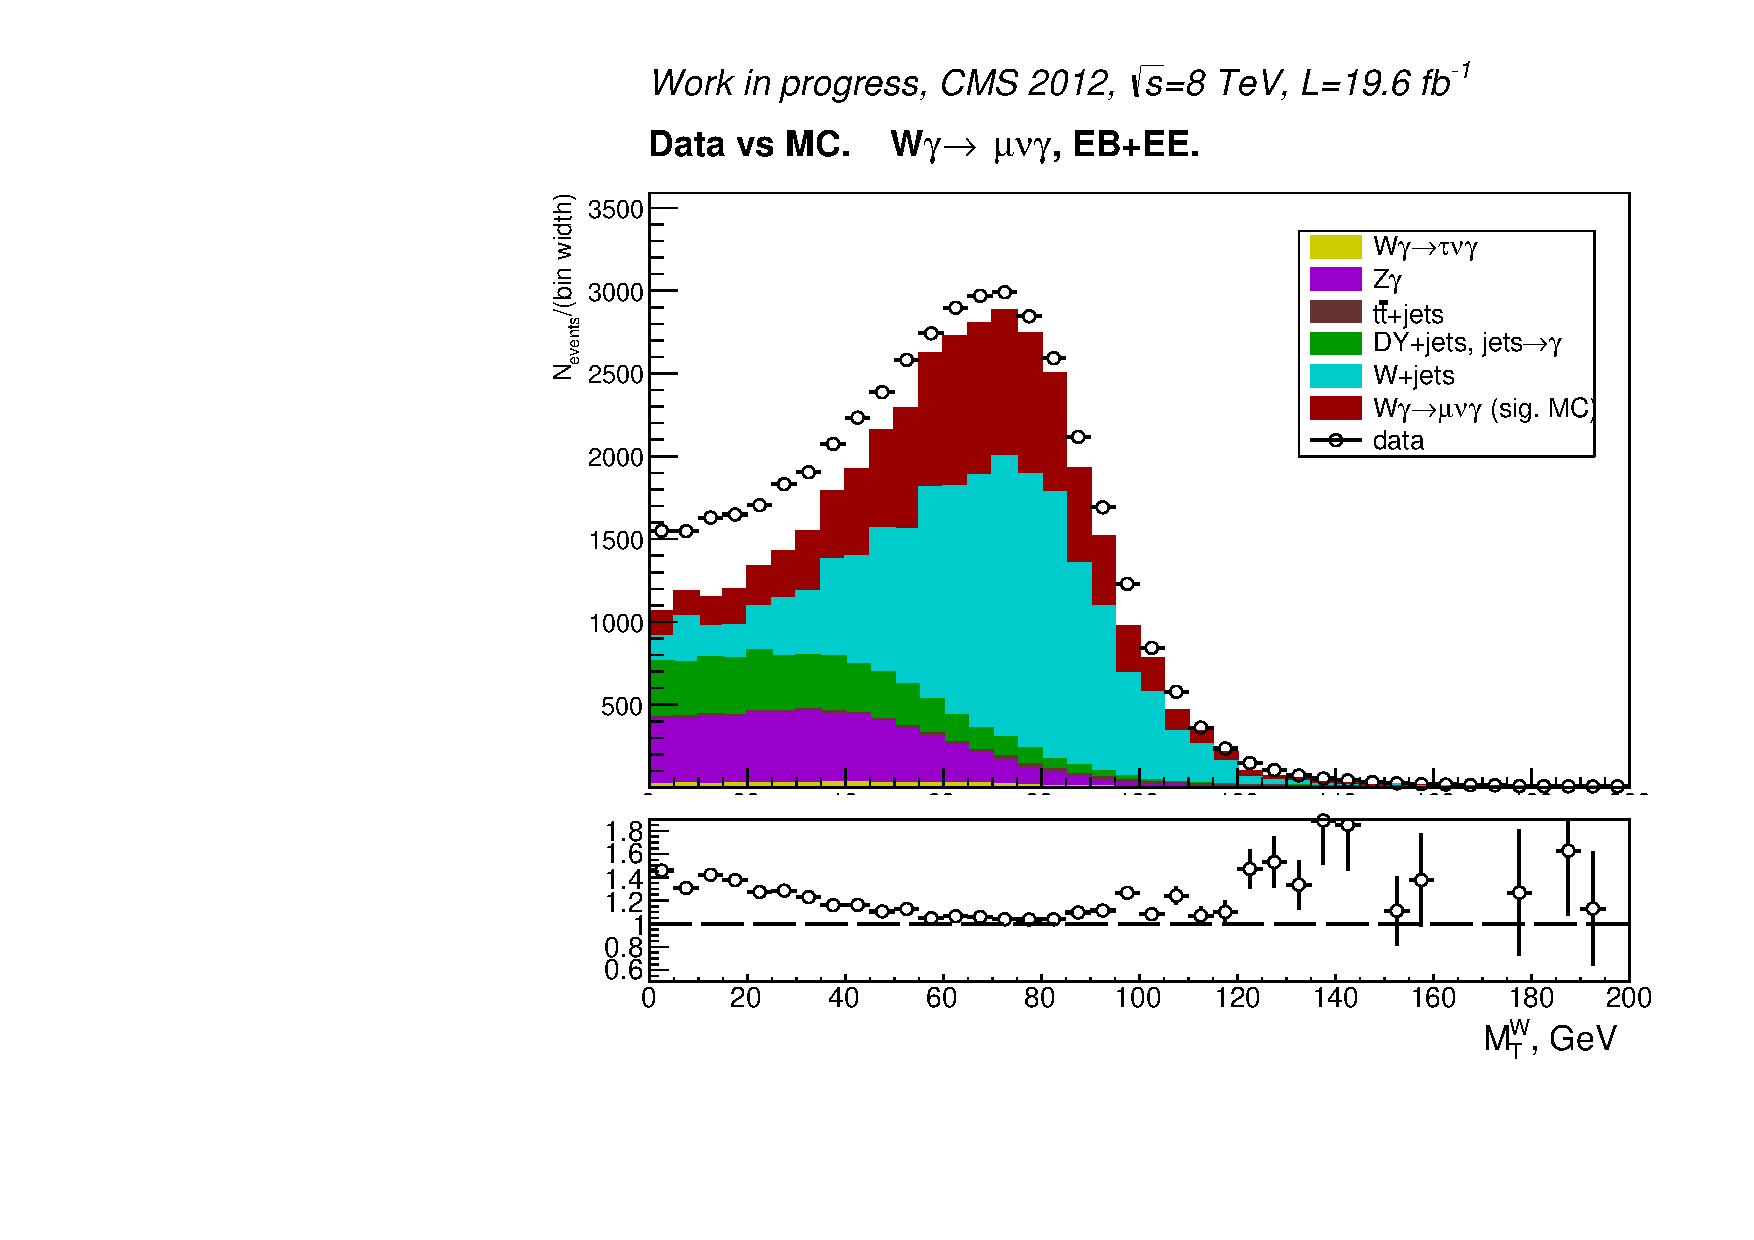
\includegraphics[width=0.45\textwidth]{../figs/figs_v11/MUON_WGamma/PrepareYields/c_TotalDATAvsMC_EtaCommon__WMtVERY_PRELIMINARY.pdf}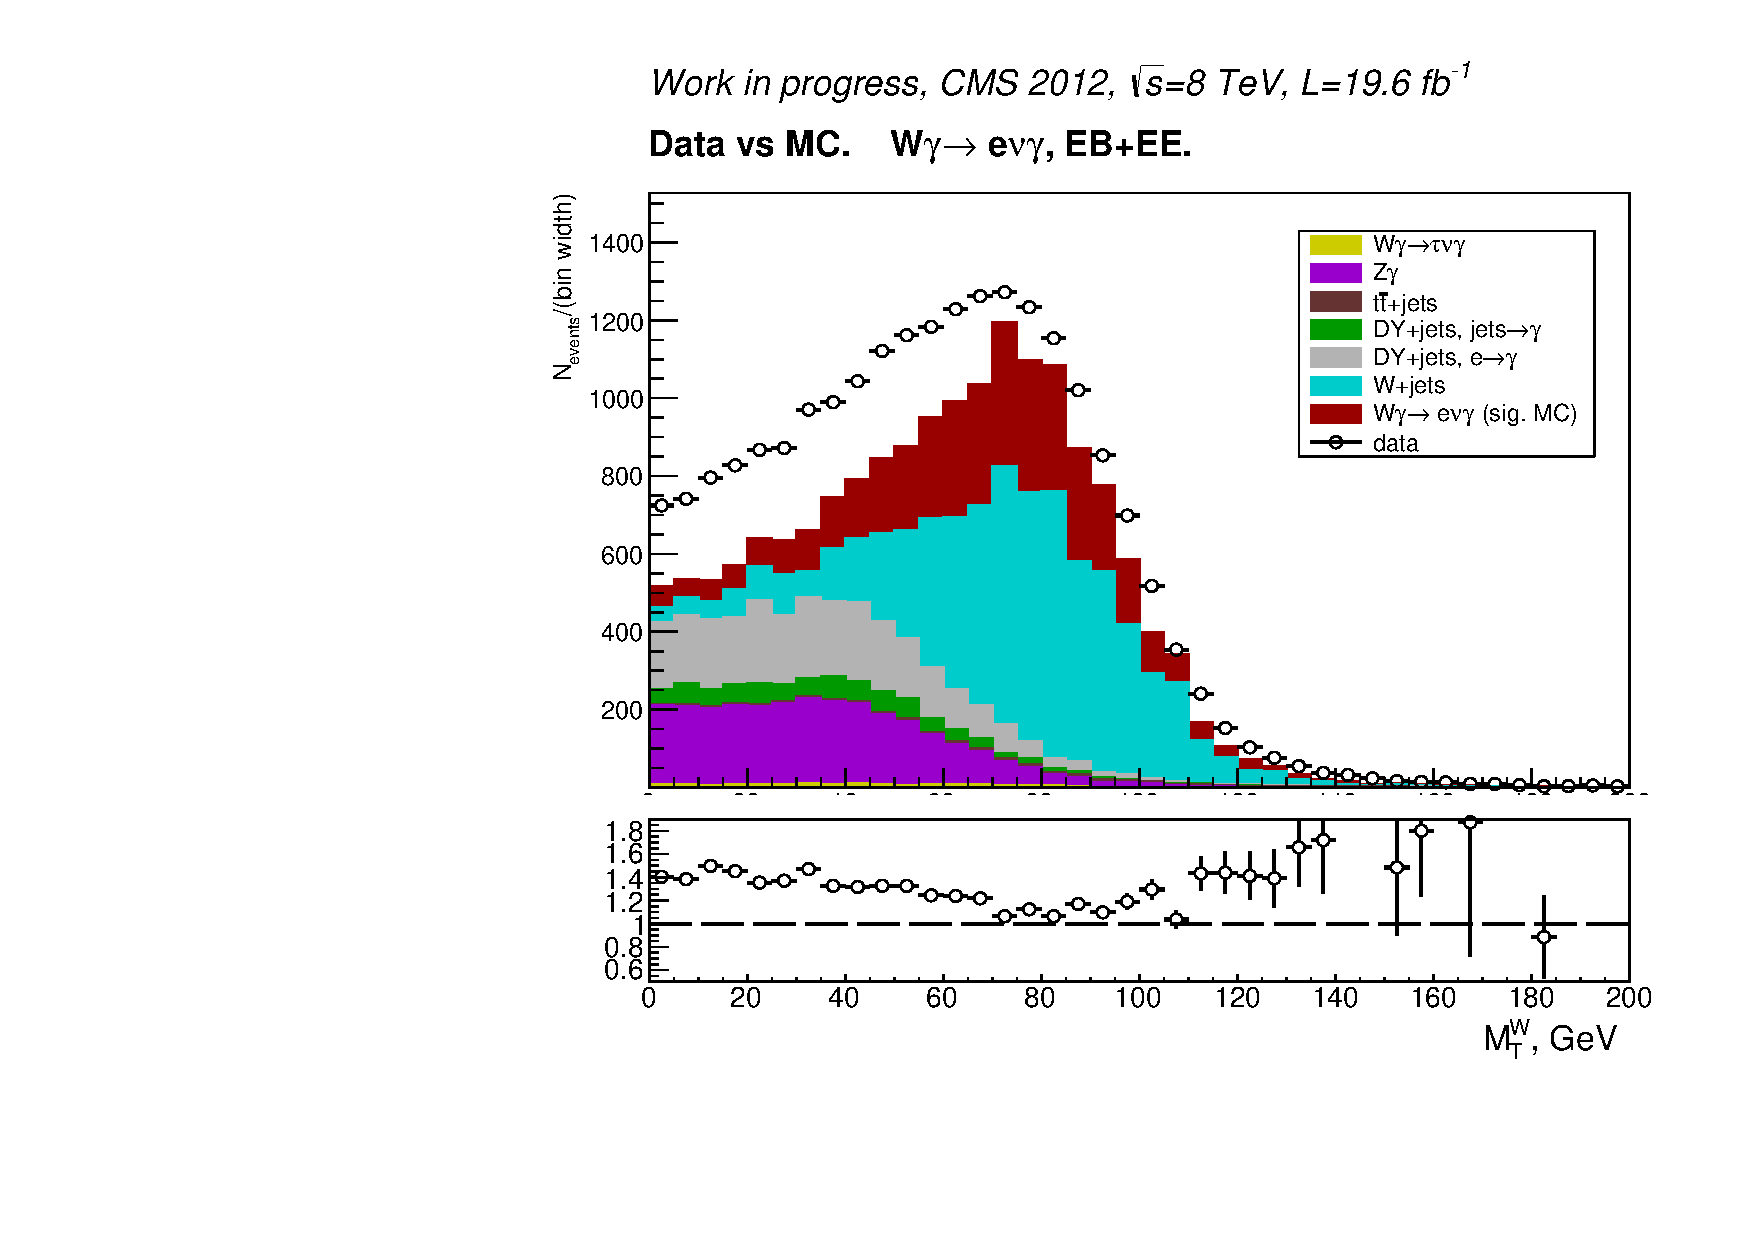
\includegraphics[width=0.45\textwidth]{../figs/figs_v11/ELECTRON_WGamma/PrepareYields/c_TotalDATAvsMC_EtaCommon__WMtVERY_PRELIMINARY.pdf}
  \label{fig:DATAvsMC_WMt}
  \end{center}
\end{figure}
\end{frame}

\begin{frame}\frametitle{Data vs MC. $M_{l\gamma}$}
\scriptsize
The selection requirement of {\bfseries{$M_{l,\gamma}<70~or~M_{l,\gamma}>110$~GeV}} is applied in the {\bfseries{electron channel}} only.
\begin{figure}[htb]
  \begin{center}
   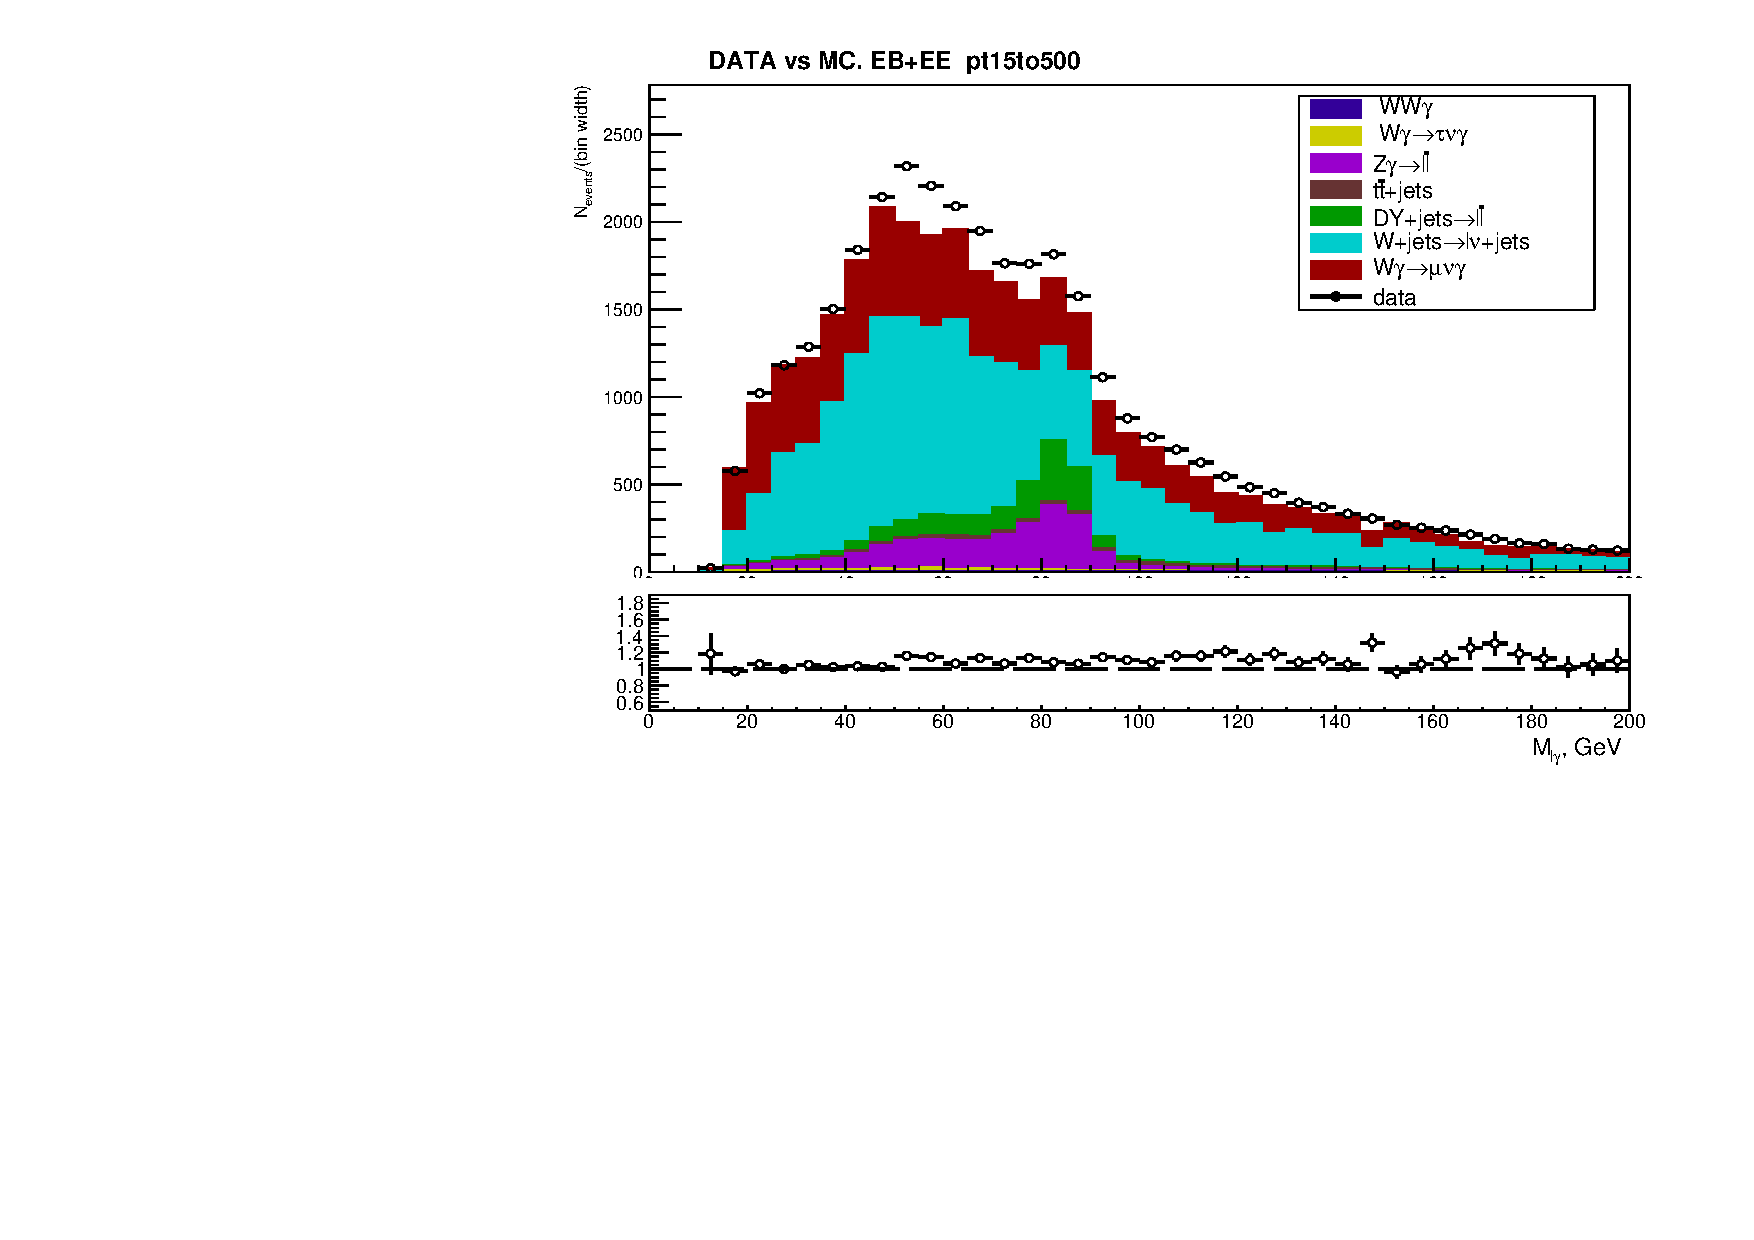
\includegraphics[width=0.5\textwidth]{../figs/figs_v11/MUON_WGamma/PrepareYields/c_TotalDATAvsMC_EtaCommon__Mpholep1_pt15to500_.pdf}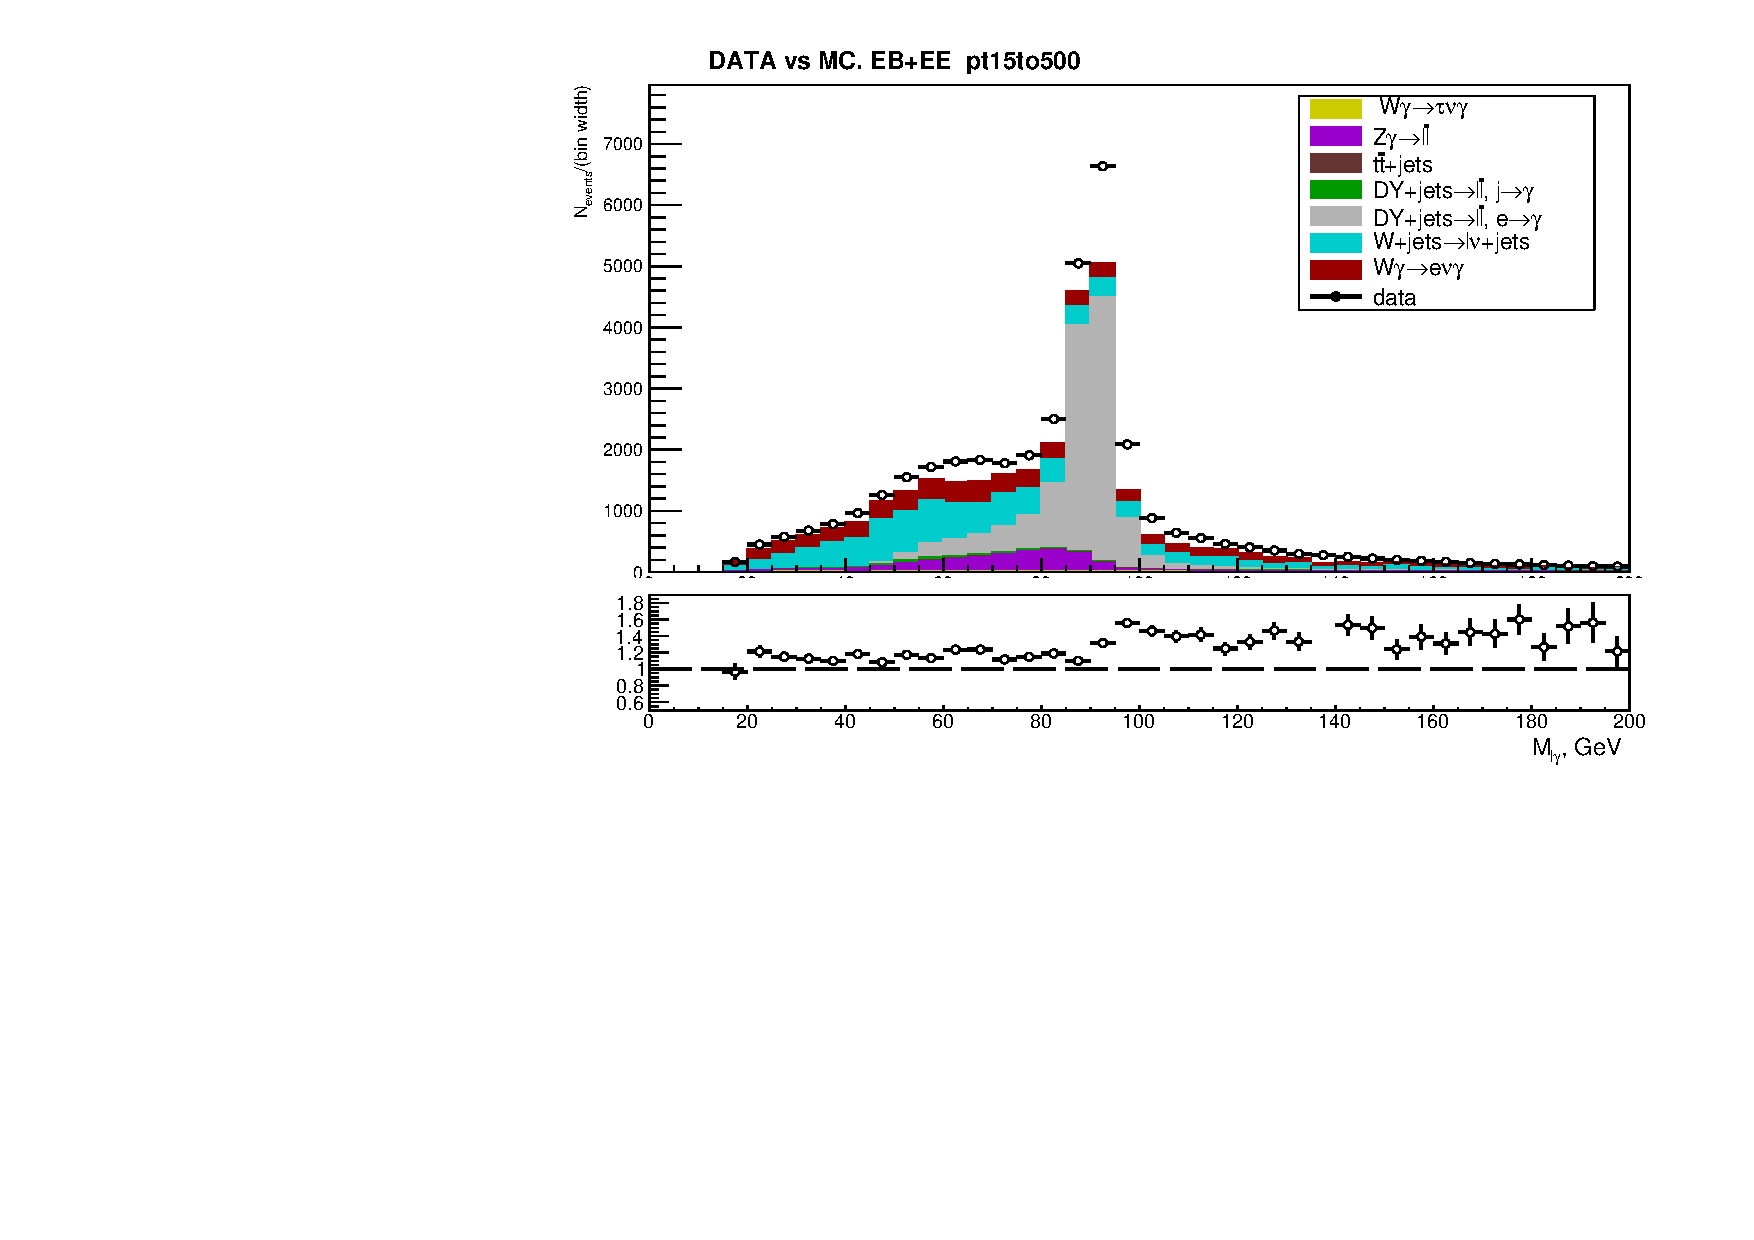
\includegraphics[width=0.5\textwidth]{../figs/figs_v11/ELECTRON_WGamma/PrepareYields/c_TotalDATAvsMC_EtaCommon__Mpholep1PRELIMINARY_FOR_E_TO_GAMMA_WITH_PSV_CUT_pt15to500_.pdf}
  \label{fig:DATAvsMC_WMt}
  \end{center}
\end{figure}
\end{frame}
